% !TEX root = main.tex
\section{Discussion}
\subsection{Impact of Advection on Spatial-Temporal Dynamics}
\begin{figure}[H]
    \centering
    \begin{subfigure}[b]{0.48\textwidth}
        \centering
        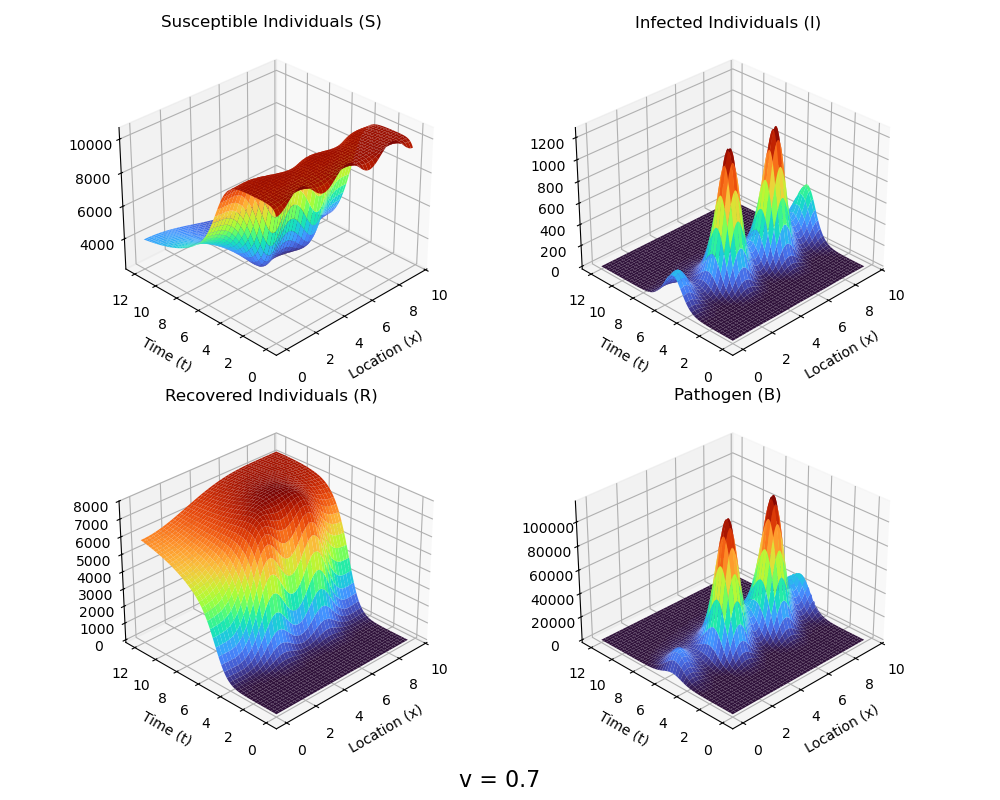
\includegraphics[width=\textwidth]{Images/v0.png}
        \caption{$v = 0.0$}
        \label{fig:v0}
    \end{subfigure}
    \hfill
    \begin{subfigure}[b]{0.48\textwidth}
        \centering
        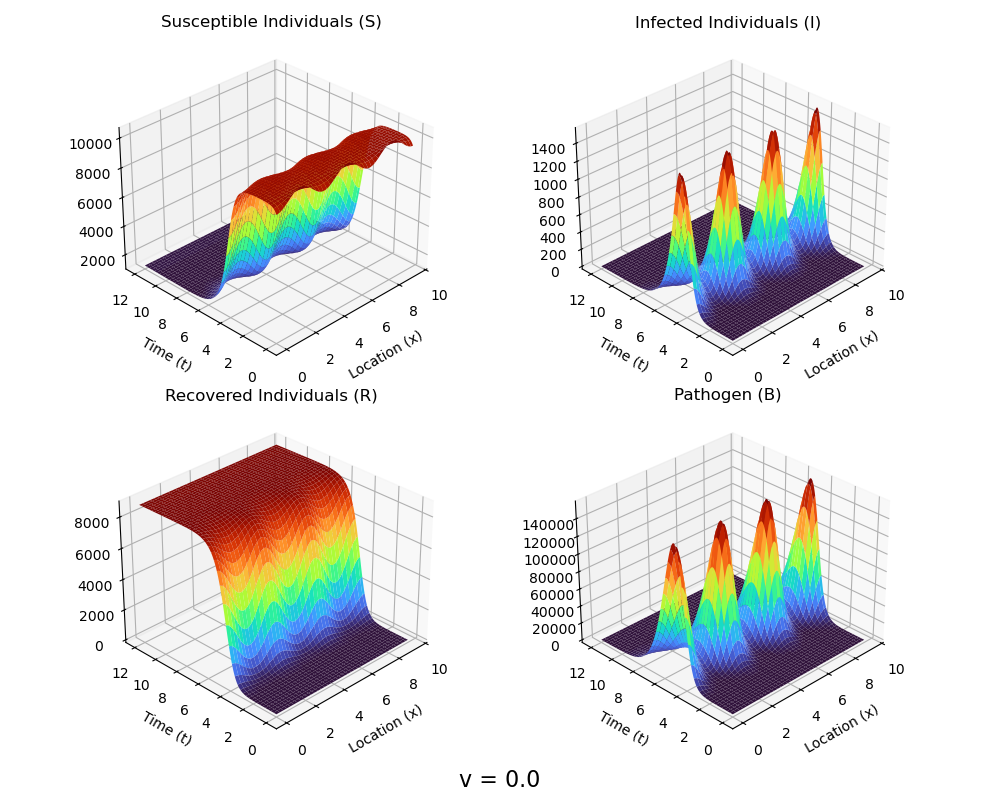
\includegraphics[width=\textwidth]{Images/v0.1.png}
        \caption{$v = 0.1$}
        \label{fig:v0.1}
    \end{subfigure}
    \caption{}
    \label{fig:advection_slow}
    %\caption{Spatiotemporal evolution of the cholera model under stagnant ($v=0.0$) and slow-flowing ($v=0.1$) conditions.}
    
\end{figure}
For Figure \ref{fig:advection_slow} we see the result off two values of $v= 0, \, 0.1$ tested in our simulation. These values were chosen to simulate stagnant water flow and slow-flowing water in the river respectively. As we can see from the 3-D graphs, they both share similar traits. For example, the spatial grid sees vary little variation as $x$ moves from $0$ to $3\pi$ towards the beginning and the end of the temporal domain. We can also see waves in the susceptible graphs as well as obvious peaks and valleys in the graphs midway through the simulated year, $t = 6$. Spatially, these occur along 4 different locations along the river. The most notable difference is in the graphs between both graphs of the pathogen at $v=0$ and $v=0.1$. The susceptible graph and infected graphs are inversely related. The graph of susceptible individuals drops significantly as time progresses while recovered individuals increases significantly as time increases. We expect these basic results as they serve as a control for the simulation. 




\begin{figure}[H]
    \centering
    \begin{subfigure}[b]{0.48\textwidth}
        \centering
        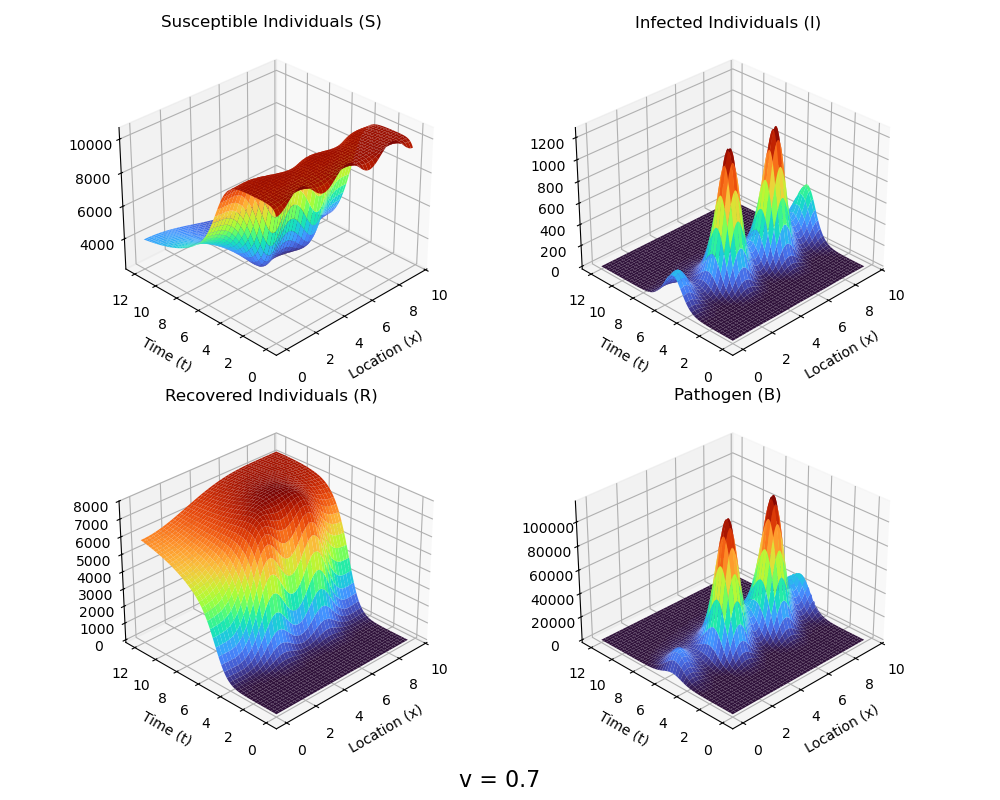
\includegraphics[width=\textwidth]{Images/v.7.png}
        \caption{$v = 0.7$}
        \label{fig:v.7}
    \end{subfigure}
    \hfill
    \begin{subfigure}[b]{0.48\textwidth}
        \centering
        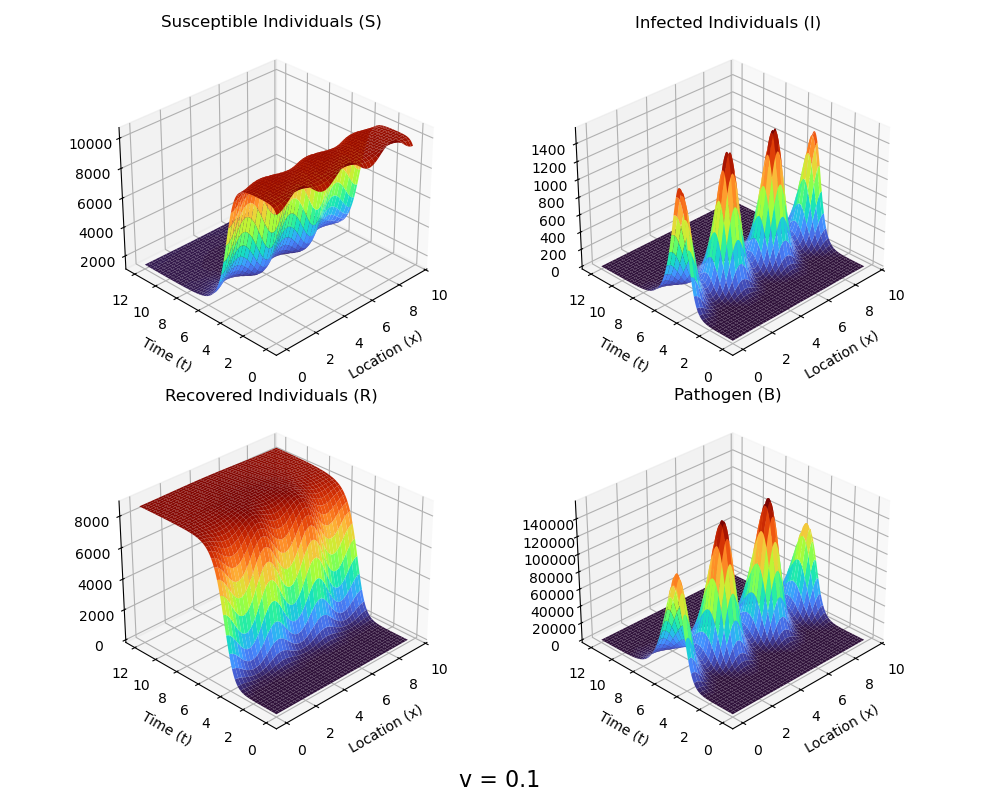
\includegraphics[width=\textwidth]{Images/v1.2.png}
        \caption{$v = 1.2$}
        \label{fig:v1.2}
    \end{subfigure}
    \caption{}
    %\caption{Spatiotemporal evolution under moderate ($v=0.7$) and fast-flowing ($v=1.2$) conditions. The advection dominates the diffusion, sweeping the pathogen downstream and causing it to accumulate against the zero-flux boundary at $x = 3\pi$.}
    \label{fig:advection_fast}
\end{figure}
\quad For Figure~\ref{fig:advection_fast}, we see the results of two higher advection values, $v = 0.7$ and $v = 1.2$, which were chosen to simulate moderate and fast-flowing river conditions, respectively. In these scenarios, advection heavily dominates diffusion. The river's current sweeps the pathogen downstream, causing a severe accumulation against the zero-flux boundary at $x = 3\pi$. Naturally as we see the concentration of the pathogen move downstream as time increases it follows that our other components follow suit. Across all subplots in Figure~\ref{fig:v.7} and Figure~\ref{fig:v1.2}, this downstream shift becomes highly pronounced. These graphical results help emphasize the importance of including the aquatic reservoir in the model (\cite{codeco2001endemic}).

\quad Comparing these faster advection rates to the slower speeds, the macroscopic effects of downstream transport become clear. As $v$ increases from $0$ to $1.2$, the rapid river flow, combined with spatial heterogeneity, creates a visible flattening effect on the upstream pathogen peaks. Biologically, the bacteria are washed away from their initial hotspots faster than they can locally reproduce. Consequently, the overall disease burden shifts toward the end of the river. This dynamic explains the spatial distribution of the human populations as time progresses. Therefore susceptible individuals are depleted much more rapidly at the downstream boundary, which in turn creates a highly concentrated, localized spike of recovered individuals in that same area.

%As we can see from the 3-D graphs, they both share similar traits. For example, the spatial grid sees vary little variation as $x$ moves from $0$ to $3\pi$ towards the beginning and the end of the temporal domain. We can also see waves in the susceptible graphs as well as obvious peaks and valleys in the graphs midway through the simulated year, $t = 6$. Spatially, these occur along 4 different locations along the river. The most notable difference is in the graphs between both graphs of the pathogen at $v=0$ and $v=0.1$. The susceptible graph and infected graphs are inversely related. The graph of susceptible individuals drops significantly as time progresses while recovered individuals increases significantly as time increases. We expect these basic results as they serve as a control for the simulation. 